\chapter{Pattern Recognition and Implementation}

% **************************** Define Graphics Path **************************

\epstopdfsetup{outdir=Chapter4/Figs/PDF/}
\ifpdf
    \graphicspath{{Chapter4/Figs/Raster/}{Chapter4/Figs/PDF/}{Chapter4/Figs/}}
\else
    \graphicspath{{Chapter4/Figs/Vector/}{Chapter4/Figs/}}
\fi


\section{Implementing the Color Space}\label{sec:ImplementingTheColorSpace}

In the previous two chapters, we have been approaching the color space design problem mathematically. Here, we will outline the practical implementation of the color space algorithm on the mobile device.

The first and most pressing consideration is limited processing power; while our mathematical approach to the algorithm design is significantly faster and more efficient than the more typical applications with commonly-used color spaces --- as will be discussed later in this chapter --- minimizing the number of clock cycles spent on continuous processes is necessary in order to ensure efficient operation. In the case of redistribution, the integer matrix transform is performed first, which puts the pixel values in the quantized working type qRange described in Chapter 2, then pixel classification is performed before any of the chromatic information is redistributed, as follows:

<pixel classification table here>

The pixel classification is performed before the redistribution because it excludes processing pixels which are of no interest based on both chromatic channels, whereas for redistribution one channel may clearly lie outside of the discard region $\lambda$ while the other could be kept or redistributed. With the pixel classifier, if one channel lies outside the discard region, the other is also of no interest since the pixel value is outside of the partitioning region, thereby avoiding unnecessary processing time spent on redistribution. The classification is straightforward within the limits on the channel values, so it isn't sophisticated like an elliptical partitioning or a probabilistic Gaussian-based thresholding; it is simply a quick way of excluding the majority of the pixel values which aren't of interest.

Once the pixels have been classified, the redistribution is performed --- which requires further processing --- or we assign a pixel value from a small set of possibilities and skip onto the next pixel values. The redistribution function is applied to the working type tRange, while the comparison and classification is done in qRange. This is because the information in tRange is compressed to avoid wasting space, and as a consequence of this it does not occupy the full data type. qRange, on the other hand, being the natural range multiplied by the quantization matrix qR, does occupy the full data type. Since the operation is simply a comparison between numbers, it is of no advantage to compress the information so tightly. Additionally, since qRange is a signed range, one could look at the bit indicating the sign and immediately tell whether or not a given value will be discarded. Once scaled to tRange, the redistribution function is applied --- which has a source range of tRange and a range dRange of the destination type --- as outlined in <insert section in Chapter 2 here>.

It should be noted that the region between the extended keep region and $\lambda$ is not especially large; for even a $5\sigma$ result, it's only tens of values wide, let alone hundreds. As such, we use a lookup table for the redistribution in our actual implementation, thus further reducing the processing overhead. It should also be noted that C++ has a lookup table threshold set to approximately 64, which makes up a quarter of a region in our case. If the redistribution region is larger than that, the error function approximation from Chapter 2 is implemented. This is mainly for future-proofing the implementation, however; given the limited size of the region, we fully expect to use a lookup table for all practical cases.

As another future concession, the facility to add pixel-based functions to the color space transform, such as the skin probability function mentioned at the end of the previous chapter, is allowed. The color space transform is a threaded process, so there is no way of knowing that the last pixel value that was processed by any given thread was an adjacent pixels, as the parallelization is handled by OpenCV's universal threading library implementations. Pixel-based functions, however, are per-pixel processes, and they come out as separate resulting channels, so they can be added to the color space transform without causing any conflicts.



\subsection{The Whiteout Blackout Algorithm.}
We need to find the point at which a chromatic value will begin to suffer from white-out and black-out. This is done by taking the corresponding RGB value for the chromatic point and illuminating and deluminating the point by shifting the channel values by the same amount and noting when each channel value becomes fully saturated or desaturated. This is done in the unit space so the results can be scaled to any working range. the algorithm for finding the theoretical values is gven in algorithm \ref{algo:TheWhiteoutBlackoutAlgorithm}. 

\begin{algorithm}[H]
 \begin{algorithmic}
  \Require{ $Ca$, $Cb$ The chromatic values}
  \State \phantom{Require}  { $iLCaCb$ the transform to LCaCb from RGB; }
  \State \phantom{Require}  {  $LCaCb$ the transform to RGB from LCaCb}
 \Ensure{  The luminosity at which black out $L_{BO}$  and white out $L_{WO}$ occur.}
 \State \phantom{Ensu} { \begin{tabular}{l}
 $Ca_{min}  \le Ca \le Ca_{max}$   \\ 
 $Cb_{min}  \le Cb \le Cb_{max}$  
 \end{tabular}  \parbox{0.65 \textwidth}{The chromatic range which could be suffering from white-out or black-out}}
 
   \State  $pnt^{RGB} \gets iLCaCb(0.5, Ca,Cb)$ \Comment{Put the point in RGB space }
   \State  $O \gets Order(pnt^{RGB}, \#1> \#2)$ \Comment{The order of the RGB channels from largest to smallest}
   \State  $\Delta WO_1 \gets 1 - pnt^{RGB}_{O(1)} $ \Comment{Iluminate to make the largest channel value saturated}
   \State  \phantom{Set} $pnt^{(RGB, WO, 1)}_{O(1)} \gets 1 $ \Comment{The point where a channel is saturated }
   \State  \phantom{Set} $pnt^{(RGB, WO, 1)}_{O(2)} \gets  pnt^{RGB} _{O(2)} + \Delta WO_1 $ 
   \State  \phantom{Set} $pnt^{(RGB, WO, 1)}_{O(3)} \gets  pnt^{RGB} _{O(3)} + \Delta WO_1 $ 
   \State  $\Delta WO_2 \gets 1 - pnt^{RGB}_{O(2)} $\Comment{Iluminate to make the second largest channel value saturated}
   \State  \phantom{Set}$pnt^{(RGB, WO, 2)}_{O(1)} \gets 1 $ \Comment{The point where two channels are saturated }
   \State  \phantom{Set}$pnt^{(RGB, WO, 2)}_{O(2)} \gets 1 $ 
   \State  \phantom{Set}$pnt^{(RGB, WO, 2)}_{O(3)} \gets  pnt^{RGB} _{O(3)} + \Delta WO_2 $ 
     
     
   \State  $\Delta BO_1 \gets  pnt^{RGB}_{O(3)} $ \Comment{Deluminate by the smallest channel value}
   \State  \phantom{Set}$pnt^{(RGB, BO, 1)}_{O(1)} \gets  pnt^{RGB} _{O(1)} - \Delta BO_1  $ \Comment{The point where a channel is desaturated }
   \State \phantom{Set} $pnt^{(RGB, BO, 1)}_{O(2)} \gets  pnt^{RGB} _{O(2)} - \Delta BO_1 $ 
   \State \phantom{Set} $pnt^{(RGB, BO, 1)}_{O(3)} \gets  0 $ 
   \State  $\Delta BO_2 \gets pnt^{RGB}_{O(2)} $ \Comment{Deluminate by the second smallest channel value}
   \State  \phantom{Set} $pnt^{(RGB, BO, 2)}_{O(1)} \gets pnt^{RGB} _{O(1)} - \Delta BO_2 $ \Comment{The point where two channels are desaturated }
   \State  \phantom{Set} $pnt^{(RGB, BO, 2)}_{O(2)} \gets 0 $ 
   \State  \phantom{Set} $pnt^{(RGB, BO, 2)}_{O(3)} \gets 0 $ 
     
   \State  $pnt^{(WO, i)}\gets LCaCb(pnt^{(WO, i)}) $ \Comment{The white-out points in LCaCb color space}
   \State  $pnt^{(BO, i)}\gets LCaCb(pnt^{(BO, i)}) $ \Comment{The black-out points in LCaCb color space}
   
   \State  $L_{WO} \gets pnt^{(WO, 1)}_1$ 
   \State  $L_{BO} \gets pnt^{(BO, 1)}_1$ 
   \State  $Ca_{min}  \gets Min(pnt^{(WO, 1)}_2, pnt^{(WO, 2)}_2, pnt^{(BO, 1)}_2, pnt^{(BO, 2)}_2 )$ 
   \State  $Ca_{max} \gets Max(pnt^{(WO, 1)}_2, pnt^{(WO, 2)}_2, pnt^{(BO, 1)}_2, pnt^{(BO, 2)}_2 )$ 
   \State  $Cb_{min}  \gets Min(pnt^{(WO, 1)}_3, pnt^{(WO, 2)}_3, pnt^{(BO, 1)}_3, pnt^{(BO, 2)}_3 )$ 
   \State  $Cb_{max} \gets Max(pnt^{(WO, 1)}_3, pnt^{(WO, 2)}_3, pnt^{(BO, 1)}_3, pnt^{(BO, 2)}_3 )$ 
     
  \State \textbf{Return} {$L_{WO} , L_{BO} , Ca_{min}, Ca_{max} , Cb_{min}, Cb_{max}$ }
 
  \end{algorithmic}
    \caption{The Whiteout Blackout Algorithm}
    \label{algo:TheWhiteoutBlackoutAlgorithm}
 \end{algorithm}
 
 The theoretical values are adjusted by 10\% to account for the auto brightness and contrast performed by the phone as described in Chapter 3 Section \ref{sec:WhiteoutAndBlackout}. We only wish to adjust the bounds away from the luminocity axis. One of the chromatic bounds will be the luminocity axis $Ca=\frac{1}{2}$ or  $Cb=\frac{1}{2}$ because this is the white or black point. Whether the bound is the upper or lower limit depends on the starting point so we define a function which performs the adjustment appropriately.
 
 \begin{equation}
 slack(x) = \begin{cases}
 (1-a) x     & x < \frac{1}{2} \\
 (1+a) x     & x > \frac{1}{2} \\
 \frac{1}{2} & x = \frac{1}{2} 
 \end{cases} \quad \text{where} \quad a = 0.1
   \end{equation}
 We can now write the condition for whether a value could have suffered from white-out or black-out. 
  \begin{multline}
 (( 0 \le L \le  slack(L_{BO}) ) \vee ( slack(L_{WO}) \le L \le 1) ) \wedge  \\
 slack(Ca_{min}) \le Ca \le  slack(Ca_{max}) \wedge  \\
 slack(Cb_{min}) \le Cb \le  slack(Cb_{max})
  \end{multline}
  
  \subsection{The Region Classification and Partitioning function}
  It is desirable to classify a pixel value after rotation but before redistribution using channel limits by how well the value fits the target and by how reliable the value is given lighting conditions. This can be done to a degree but it is necessary to assume reasonably uniform lighting conditions. The pixel values are classified by chromatic value as either inside the target region or outside in both axis dividing the chromatic plane into nine regions fig \ref{fig:PartitioningRegions}. A rudimentary partitioning is performed by assigning 8 constants to the values outside the region around the mean. The luminosity is always evaluated because all that is required is a scaling from qRange to the destination range dRange. 
  
  \begin{figure}[h!]
    \centering
      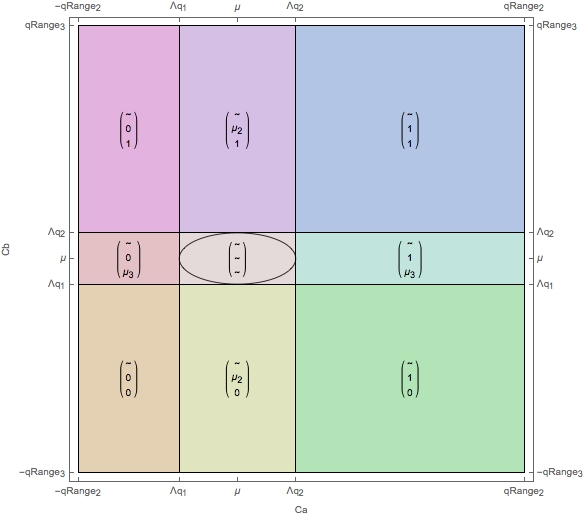
\includegraphics[width=0.80\textwidth]{Chapter4/Figs/PartitioningRegion.jpg}
      \caption{The Regions in the chromatic space. ~ Indicates values which will undergo redistribution. Regions outside the target area are allocated extreme values at the edge of the color space}  \label{fig:PartitioningRegions}
  \end{figure}
  
  \subsection{Floating the Mean}
  Different lighting conditions can affect the detected pixel color. Not accounting for strongly colored light the affect of different lighting conditions is to increase or decrease the saturation of the color. The distribution is relatively unaffected in orientation or variance meaning that lighting conditions can be accounted for by adjusting the mean. 
  \newcommand{\newMean}{\widetilde{\mu}}
  The algorithm adjusts to ambient lighting by first taking a reference image centered on a patch of skin and finding the mean in the LCaCb colorspace. This new mean $\newMean$ is then used in the current instance of the algorithm. It is adventitious to keep the mean adjustable in the routine so this is implemented by introducing  an adjustment parameter $\delta\mu$ to the routine where $\newMean = \mu + \delta\mu$. The algorithm assumes that the adjustment is small enough that the distribution function retains the same shape aside from a translation along the axis. This allows the distribution parameters to be adjusted by simply shifting them by $\delta\mu$. 
  
  \begin{equation}
  \begin{aligned}
   \widetilde{\lambda}_1 & = \lambda_1 + \delta\mu &  \widetilde{\lambda}_2 & = \lambda_2 + \delta\mu \\
   \widetilde{\omega}_1 & = \omega_1 + \delta\mu &  \widetilde{\omega}_2 & = \omega_2 + \delta\mu 
  \end{aligned} \quad \text{Where} \quad \lambda_1 < \delta\mu < 1 - \lambda_2
  \end{equation}
  
  \subsection{The Colorspace Algorithm as Implemented}
  Here we present the colorspace algorithm in a way which most closely resembles the C++ code. The construction of the colorspace object is described at the end of chapter 2 here the operation of the algorithm is described.
  
  First we determine the form of the distribution function for a working type tRange with The source range $srcRange=2^n$  and destination range $dstRange=2^m$ expressed in terms of their bit depths.
  
  \begin{gather*}
   \begin{aligned}
    \delta  &= \frac{ \sqrt{2} }{ \sigma \sqrt{\pi }  \left(\Sigma^+-\Sigma^-\right)} & 
   K & =  2^{m-n}  & 
   \Sigma^- &= \text{erf}\left(\frac{\mu -1}{\sqrt{2} \sigma }\right) &
   \Sigma^+ &= \text{erf}\left(\frac{\mu }{\sqrt{2} \sigma }\right) 
    \end{aligned} 
  \end{gather*}
  The length of the axis $\tRange$ after rescaling is given by \ref{eq:CombinedRotationRange}, and the axis limits are easily found along with 
  the compression ratio $\kappa$ (\ref{eq:newCompressionRatio}).
  \begin{gather*}
  \begin{aligned}
   \tRange(\theta,\mu,\sigma)   & =  \mathbf{l} \; 2^n \quad&\quad
  \mathbf{l}  & = \min\left\{ 2^{m-n}\delta(\mu,\sigma) \right. ,  \left. \mathbf{L}(\theta) \right\} 
   \end{aligned} \\
   \begin{aligned}
    \tMin(\theta,\mu,\sigma)   & =
   \begin{pmatrix}
      0 \\
    -\mathbf{l}_2 \; 2^{n-1}  \\  
    -\mathbf{l}_3 \; 2^{n-1} \\  
   \end{pmatrix} \quad & \quad
    \tMax(\theta,\mu,\sigma)   & =
   \begin{pmatrix}
    \mathbf{l}_1 \; 2^n  \\
    \mathbf{l}_2 \; 2^{n-1}  \\  
    \mathbf{l}_3 \; 2^{n-1} \\  
   \end{pmatrix} 
   \end{aligned}
  \end{gather*}
  
  
  \begin{equation*}
  \Scale =
   \mathbf{l} \otimes
  \begin{pmatrix}
    \frac{1}{3} \\
   2^{1-n } \\
   2^{1-n }  \\
  \end{pmatrix}    \\
  \end{equation*}
  
  
  Substituting into the distribution function \ref{eq:disFunction} gives us
  
  \begin{equation}
\textbf{dis}(x) =  -\frac{2^n \left(\text{erf}\left(\frac{2 \mu +1}{2 \sqrt{2} \sigma }\right)+\text{erf}\left(\frac{2^{1-2 n} x-\mu }{\sqrt{2} \sigma }\right)\right)}{\text{erf}\left(\frac{2 \mu -1}{2 \sqrt{2} \sigma }\right)-\text{erf}\left(\frac{2 \mu +1}{2 \sqrt{2} \sigma }\right)} \quad \textbf{where} \quad
\begin{array}{rl}
qMin < & x  < qMax \\
0 < &\mu <1\\
0 < &\sigma <1
\end{array}
  \end{equation}
  
  This form takes the result of the rotation directly however we wish to add the flexability to adjust the mean and to use a lookup table for the values. It is desirable to keep the lookup table as short as possible. The maximum compression of the information without loosing relevant information is given by compressing to tRange. The number of values in the lookup table can be reduced by scaling $x$ by a range qtRange which is chosen to balance lookup table size and computational scaling efficiency.  Noting that $\mathbf{l} <2$, qRange is chosen to be equal to tRange as if $\mathbf{l} =2$ which means that qtRange is a power of two allowing the scaling to be performed by bit shifting the value of $x_{qt} = x \ll n-2$ . Adjusting the mean changes the bounds on the region to be redistributed such that the form of the function does not change. For this reason we also define $x$ relative to the bounds which allows the same lookup table to be used regardless of any adjustment to the mean.
  
    \begin{equation}
  \textbf{dis}(x) =  \begin{cases}
    \textbf{disLU}((x-\Lambda_{1}) qtRange)  & \Lambda_{1} < x < \Omega_{pq1} \\
  \textbf{disLU}((x-\Omega_{pq2}) qtRange)  & \Omega_{pq2} < x < \Lambda_{q2} \\
  \textbf{dis}(x)  & \text{Otherwise}
    \end{cases} \quad \text{where} \quad 
    qtRange = \left(\begin{smallmatrix}
    \cdots \\ 2^{2-n}\\2^{2-n}
    \end{smallmatrix}\right)
    \end{equation}
  
  Aside from these refinements the algorithm presented in Chapter 2 is used to perform the rotation and redistribution as described. The algorithm proceeds as follows.
  
  \begin{itemize}
  \item Interactively find an adjustment to the mean  $\delta\mu$. .
  \item Set the new distribution parameters
  \item Rotate the pixel value with the $\qR$ matrix. $ pxl_{q} = \qR \cdot pxl_{RGB}$ then $ \frac{- qRange}{2} < pxl_{q} < \frac{ qRange}{2}$
  \item Partition the rotated values to avoid unnecessary processing of irrelevant information.
  \item Apply any user supplied per-pixel functions to the rotated value and add as extra channels.
  \item Redistribute the rotated values into the destination type.
  \item Apply and user supplied per-pixel functions to the redistributed values.
  \end{itemize}

\section{Pattern Recognition routines}
In this section pattern recognition routines which use the new color space are presented and discussed.

\subsection{Improved Contour Detection}\label{sec:ImprovedContourDetection}

OpenCV's findContours method takes a binary image and finds the contours in that binary image. However, the problem with this method is that we're thresholding on chromatic values, i.e. using color information to break up the color information into blobs off of which we're finding the contours. This doesn't take into account the white-out and black-out, which was noted previously. It's straightforward to define regions in the image which are succeptible to white-out and black-out using the luminosity channel. This is done by taking a high and low threshold off the luminosity channel, thereby producing a binary image, which is 1 in the valid region, and 0 otherwise.

We take that, and we add it to our thresholded chromatic channel, which produces a 2-bit image. For this purpose, a 2-bit data type was added to OpenCV. The question then is how to use it. Essentially, we have four different states: values which are neither the right color nor in the right region; values which are possibly the right color, but because they're outside the valid region, they've potentially suffered from white-out and black-out and as such they are not reliable indicators for either the start of an edge or the end of an edge; values which are in the right region, but the wrong color, and we are certain that they are not skin; and finally, values which are in the valid region and are of the right color.

The Canny edge detector method is perfect for implementing a decision by setting a high threshold --- our strong criteria --- in the right region in the right color, and a low threshold so that it will continue following an edge across values which are in the invalid region. Whichever value we set the low threshold to depends on the state of the image; we use a lower value if there is ambiguity and a higher value if the result is fairly accurate:

\begin{center}
\begin{tabular}{|c|c|c|c||c|c|}
\hline
\multicolumn{2}{|c|}{Image} & Color & Region & \multicolumn{2}{|c|}{Bit}\\\hline
0 & 0 & 0 & 1 & Color & XAND(Color, Region)\\\hline
0 & 1 & 0 & 0 & Color & XAND(Color, Region)\\\hline
1 & 0 & 1 & 0 & Color & XAND(Color, Region)\\\hline
1 & 1 & 1 & 1 & Color & XAND(Color, Region)\\\hline
\end{tabular}
\end{center}

\begin{figure}[h!]
  \centering
    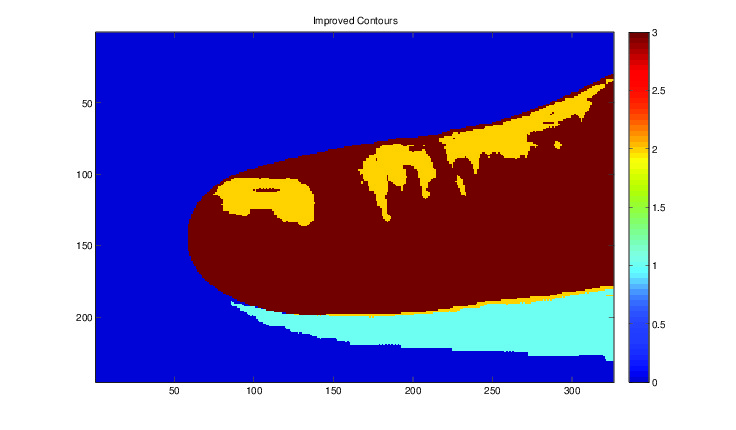
\includegraphics[width=0.70\textwidth]{Chapter4/Figs/2bitImage.jpg}
    \caption{The improved contour method in action.}\label{fig:2BitImage}
\end{figure}

\section{Fingertip Descriptor}\label{sec:FingertipDescriptor}

Given that the SURF method fails to find any sort of reliable, small area features, we need a descriptor so we can accurately align points on the fingertip between successive images in the video stream. We need to do this because otherwise, any difference between the frames will be overwhelmed by physical movement of the digit rather than movement of the blood inside the digit. For this reason, we target the most stable portion of the finger: the nail. We have quite accurate tracking of the tip, so it's quite simple to place a point fairly centrally on a nail with no other information other than the position of the tip. We apply the Canny edge detector and find the edges which are radially located around that point. The radial edges are detected, which are used to align between frames. Essentially, they can be broken into four lines; two down the side being relatively straight. But it depends on the individual, and the digit. However, we know we're looking for something with a certain curvature, as well as the rough positions of the lines along the edges.

For each of those four lines, we have an orientation and a curvature, as well as the distance between the opposing lines. So, using that descriptor, we have the next frame, and in the new frame, we apply the Canny edge detector and detect four lines with similar characteristics. Given those edges, we can produce our best estimate, minimizing the difference between this frame and the previous one, in terms of their orientation and position. Based on this, we can work out a shift if there's been a change in position or orientation of the fingertip.

Because we're going from one frame to another in a video stream, the descriptor is sufficient to overlay the frames accurately to within a few pixel widths. Brute force feature matching can be used as a further refinement if necessary. For the purposes of detecting a finger press, however, this was not found to be necessary.

\section{Putting it All Together}\label{sec:PuttingItAllTogether}

So far, we have said little about how we actually intend to detect a digit being pressed on a surface. Although a significant amount of discussion has been presented to do with the optimization --- at least in terms of the data types and the underlying maths --- mostly to do with the color space transform. We have said even less about the size of the images captured or the framerate at which the processing is required. These are important considerations for designing practical code, especially for application in a mobile device.

\subsection{Detecting a Finger Press}\label{sec:DetectingAFingerPress}

In the previous section, we presented several algorithms which perform steps in the task. However, we now need to put them together and fill in the gaps which link each important step together. Assumptions and simplifications which we have allowed ourselves in this work which is intended only to be a proof of concept rather than a fully-fledged application. To this end, we have decided to simplify the requirements and --- although there is no compelling reason why we could not use, say, convex hull and defects to detect the fingers, or even a full hand --- we're only going to consider the case where one digit is presented to the routine in a controlled environment:

The first step in the algorithm is to select a human and a camera. With this done --- using the same camera as will be used by the application --- we gather statistics for a particular individual's skin, trying to vary the lighting conditions so as to give us as representative a data set as possible. From this, a color space is designed and the relevant transforms and such are instantiated for that particular individual.

The next step is to collect the finger features and instantiate the feature detectors using the Canny-edge-based descriptor for each of the individuals' digits.

Now we start the application: it turns on the camera and waits for movement. After the movement starts, it continues to wait until that movement slows, which is the first indicator that a surface is being touched. Here we assume that we are trying to detect static presses, so no pressing and dragging is considered. We look at a higher resolution frame, process that frame into the skin color space for the individual in question. 

Now we perform our shape detector, which looks for a finger-shaped object, finds the tip, creates rectangular bounds for the tip, and then takes an even higher resolution frame. (But only for the tip of the potential finger.) This image --- cropped to the tip of the digit --- is then sent to the feature detecton algorithm, which then uses the Canny edge feature method previously described and attempts to identify the digit by applying the known descriptors for the individual's nail.

These steps are relatively slow, but --- once applied --- the algorithm now only tries to fit one feature descriptor and simply tracks the assumed small movement of the tip during a press. Due to the slow nature of these steps, it's required that the camera buffers a few frames after the motion stops, otherwise the finger press may miss the processing window. It is at this stage that the algorithm to detect the finger press really starts.

Now that the fingertip has been located, the algorithm crops the fingertip before forming the color space transform, which saves a significant amount of processing time. We now define a larger cropping region, and a tight cropping region. The larger of the two cropping regions is used initially to ensure that the entire tip of the digit is captured in subsequent frames, as this cropping region will not vary during the finger press detection stage of the algorithm. Inside the cropping region, a second rectangular region is defined, which is centered using the feature detection, ensuring that the frames are aligned with the true outline of the digit and not the outer pixels. Any change in the tighter frame will be due to the mechanical action on the digit changing its visual appearance.

The tightly-cropped region from each frame is held in as high a resolution as possible, and the absolute distance between each successive frame is calculated in this region. It was discovered that the color channel corresponds to the major axis of the 2D Gaussian fit to the chromatic space. It has been found that a finger press changes the chromatic values in the end of the digit sufficiently for this to register clearly in this region. For the purposes of this project, this difference is calculated and output as an image. However, for the actual application, all that is required is a measure of the size of the change in the chromatic space.

\begin{figure}[h!]
  \centering
    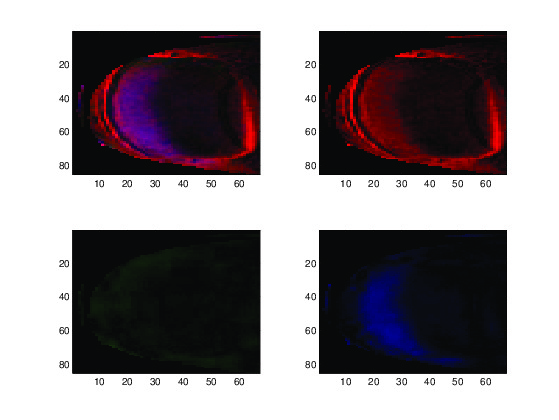
\includegraphics[width=0.90\textwidth]{Chapter4/Figs/jThumb_Final_Proof.jpg}
    \caption{The difference in the skin color space between successive frames during a finger press. (Or in this case, a thumb.)}\label{fig:FinalProof}
\end{figure}

The second indicator for a finger press was found around the center of the pad of the digit. The distance to the convex hull --- which outlines the edge of the digit in the frame --- was noted to move away from the centered reference point. This is because the nail does not significantly deform under mechanical stress, however the soft tissue underneath does. This provides a second level in the metric for detecting a digit press.

The algorithm now decides based on thresholds which could be trained, but in the present implementation were set manually, one on the chromatic difference in the feature region (i.e. the nail), and the second on the contour from the shape detection. The output of each combined to produce a sound, the idea being the harder you press, the louder the noise.

The final step is to detect when the digit starts moving again. Failure of the feature detector to re-align the small frame makes the algorithm start tracking motion again. It looks at the low-resolution frames and sees if significant movement is occurring in the larger frame. It should be noted that the algorithm does not process outside of the larger cropped region during the finger press detection phase.

\section{Skin Detection}\label{sec:SkinDetection}

With the image in the skin color space, skin detection is a significantly simplified problem; the average skin color is at the halfway point in both of the chromatic channels and the Gaussian distribution has already been applied, meaning that performing an elliptical thresholding in the normal color space is equivalent to a rectangular thresholding in the skin color space. The probability distribution can be obtained by combining the distributions in each chromatic channel. Because the thresholding levels in each channel are equivalent to the same points on the Gaussian, they can be straightforwardly combined, and then a single threshold used on the one resulting channel. This can be done by subtracting $\frac{1}{2}$ from both channels, squaring them, then adding them together.

The next step is to identify the skin. For the purposes of this project, we're searching for a skin-colored object of a specific shape: a finger that comes into the frame, presses down on a surface, then exits the frame. One of its properties is that it meets the edge of the frame, appearing as a rectangle with a rounded end which --- on occasion --- can appear slightly bent due to the viewing angle or pressure placed on the finger as it presses down on the surface. But there's a limit to how great that deflection can be in the image.

In order to find this shape, we begin by finding the contours in the binary probability image. This can be achieved by using the "findContours" method in OpenCV, which finds the contours and returns them as a vector of points. In the skin color space, finding the contours around the finger is very simple.

\begin{figure}[h!]
  \centering
      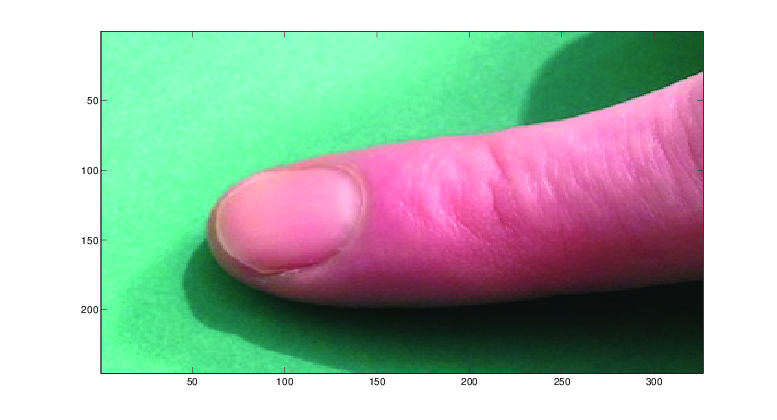
\includegraphics[width=0.45\textwidth]{Chapter4/Figs/imgJIndex1.jpg}
    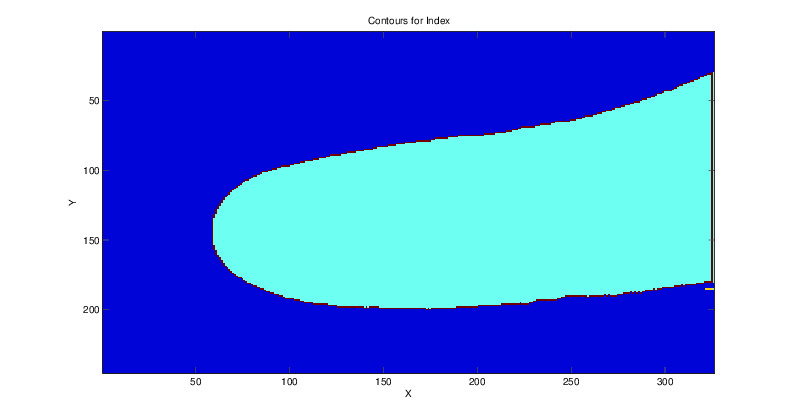
\includegraphics[width=0.45\textwidth]{Chapter4/Figs/indexContours.jpg}
    \caption{Finger contours in the probability image.}\label{fig:IndexContours}
\end{figure}

Once the contours have been identified, a rectangle is drawn around the finger using OpenCV's "rectangle" method, with the tip of the finger touching one of its sides. Next, lines are drawn along the sides of the finger using the "line" method, and a convex hull identifies the semicircular fingertip, again using an OpenCV method, in this case "convexHull." This produces a set of verteces which allow us to locate the fingernail, at which point we highlight it with a square drawn using the "rectangle" method once more. The fingernail image within this square is then sent to the edge detector method for further processing. (See Figure 2.17.)

It should be noted that --- in the finger images in Figure~\ref{fig:IndexContours} --- the finger is deformed slightly due to the application of pressure on a flat surface, as was discussed previously. This doesn't necessarily share the same orientation as the tip. This can be remedied by taking the portion of the image highlighted by the rectangle and performing the operation again, thereby producing a rectangle which is properly oriented with the fingertip.

Once the fingertip has been identified, its features are obtained using the SURF algorithm method provided by OpenCV's SURF class. An initial attempt was made to use the library functions in OpenCV, however the high resolution and the relative uniformity of the fingertip resulted in no stable feature points being automatically detected. The initial idea was to allow the automatic descriptor generator to use a set of aligned frames and the idea was to keep the features which were stable in time and space. (i.e. Present in every frame and in the same location.) This attempt was unsuccessful, so a bespoke method was designed instead.

\begin{figure}[h!]
  \centering
    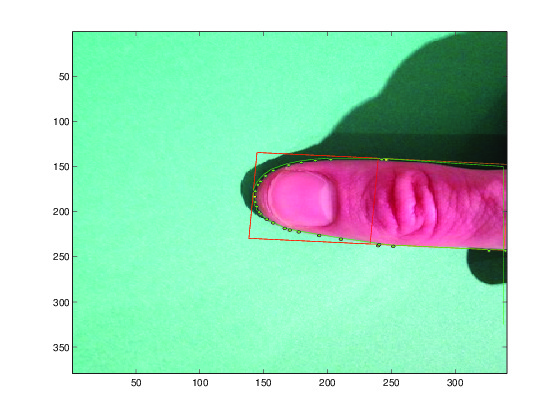
\includegraphics[width=\textwidth]{Chapter4/Figs/shapeDetection.jpg}\label{fig:shapeDetection}
    \caption{Shape detection in action.}
\end{figure}

\begin{figure}[h!]
  \centering
    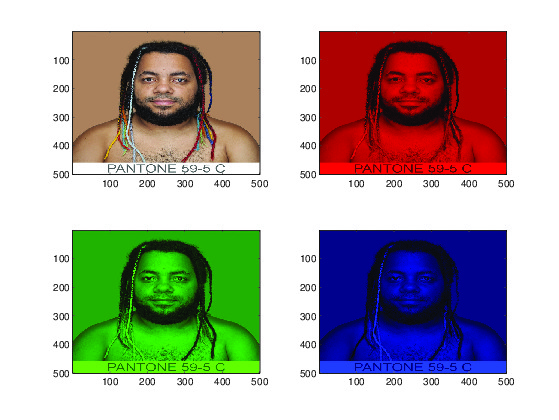
\includegraphics[width=\textwidth]{Chapter4/Figs/rainbowmanRGB.jpg}
    \caption{RGB channels.}
\end{figure}

\begin{figure}[h!]
  \centering
    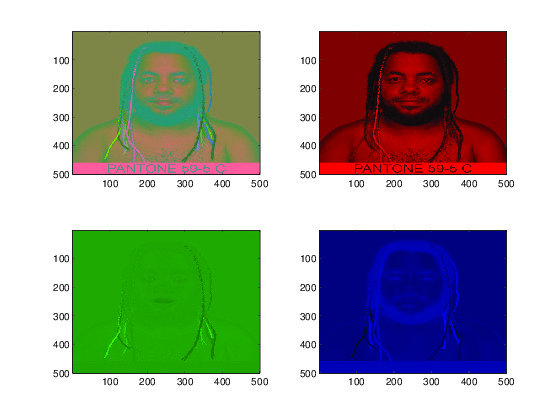
\includegraphics[width=\textwidth]{Chapter4/Figs/rainbowmanRotated.jpg}
    \caption{Rotated color space.}
\end{figure}

\begin{figure}[h!]
  \centering
    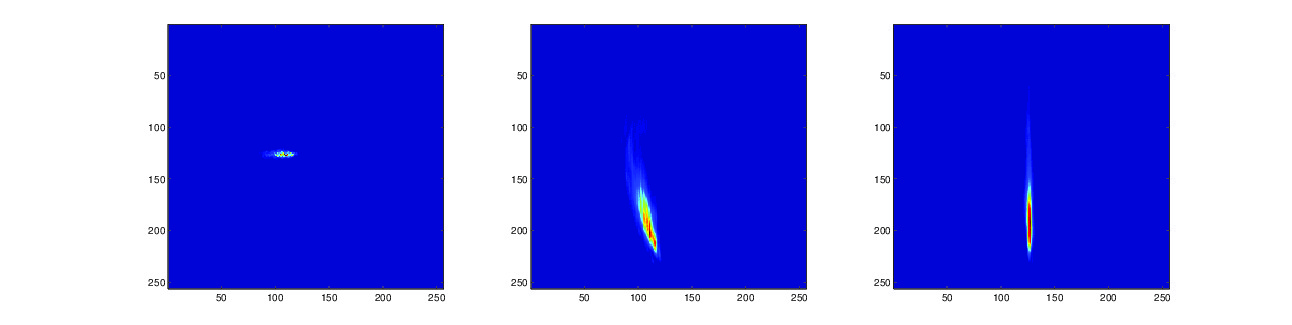
\includegraphics[width=\textwidth]{Chapter4/Figs/binsFinal2.jpg}
    \caption{Final bins.}
\end{figure}

\begin{figure}[h!]
  \centering
    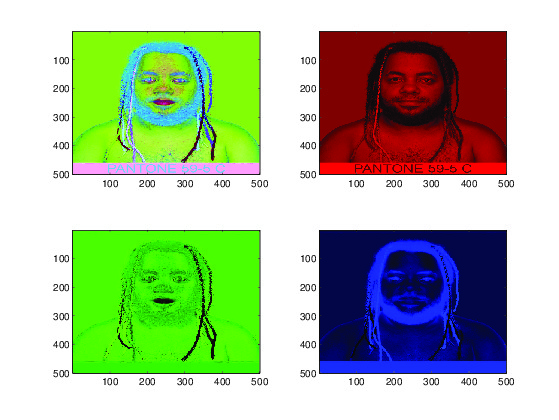
\includegraphics[width=\textwidth]{Chapter4/Figs/rainbowmanRotatedScaled.jpg}
    \caption{Rotated and scaled color space.}
\end{figure}
